\documentclass{zkdl-presentation-template}
\usepackage[utf8]{inputenc}
\usepackage[english,ukrainian]{babel}

% -- Including some standard packages --
\usepackage{graphicx}
\usepackage{soul}
\usepackage{hyperref}
\usepackage{colortbl}
\usepackage{dsfont}

% Tikz
\usepackage{tikz}
\usetikzlibrary{matrix,positioning,fit,backgrounds,intersections}

% -- Cross signs --
\usepackage{pifont}% http://ctan.org/pkg/pifont

\title{\textbf{Задача сегментації для медичних зображень: U-Net Архітектура}}
\author{Захаров Дмитро}
\date{26 листопада 2024 р.}

\titlegraphic{
    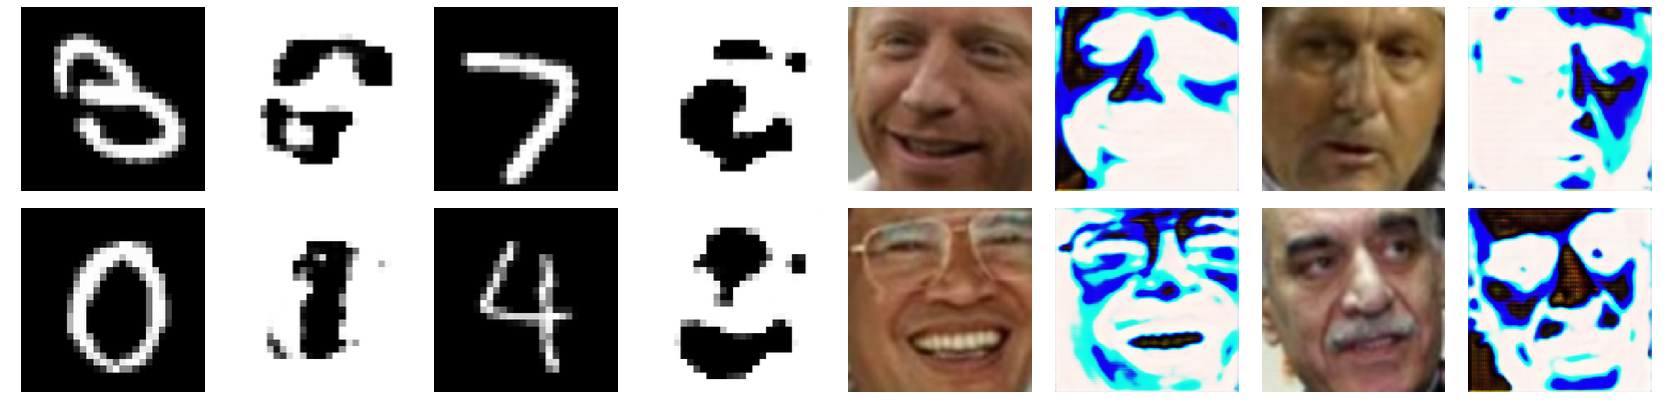
\includegraphics[width=0.7\textwidth]{images/preview.png}
}

\expandafter\def\expandafter\insertshorttitle\expandafter{%
  \insertshorttitle\hfill%
  \insertframenumber\,/\,\inserttotalframenumber}

\AtBeginSection[]{
  \begin{frame}
  \vfill
  \centering
  \begin{beamercolorbox}[sep=8pt,center,shadow=true,rounded=true]{title}
    \usebeamerfont{title}\insertsectionhead\par%
  \end{beamercolorbox}
  \vfill
  \end{frame}
}

\begin{document}
	\frame {
		\titlepage
	}
 
	\begin{frame}{План}
        \tableofcontents
    \end{frame}
	 
	\section{Вступ}
    \subsection{Задача сегментації медичних зображень}
	\begin{frame}{Задача сегментації}	
		\begin{block}{Задача сегментації}
            Зазвичай, маючи зображення $X$, виділяє регіони (розбиття) $\mathcal{R}_1,\dots,\mathcal{R}_C$, що відповідають певним ознакам.
        \end{block}
        
        \begin{figure}
            \centering
            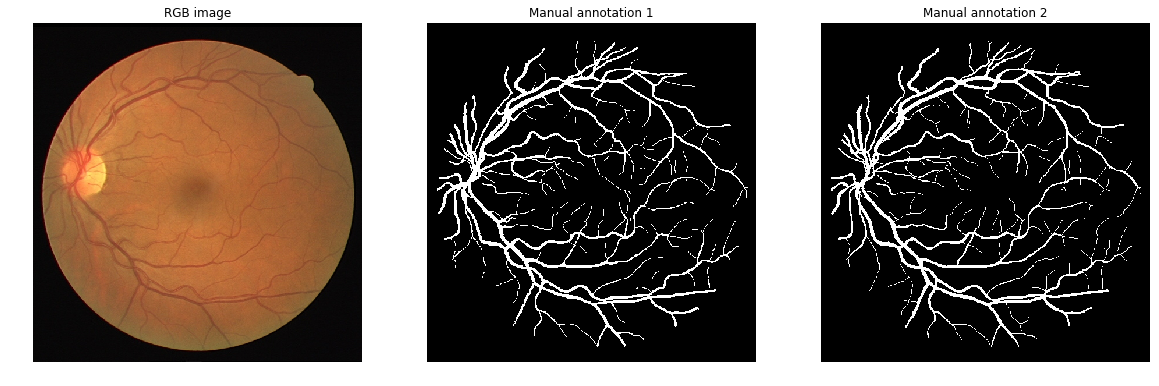
\includegraphics[width=\textwidth]{images/retinal-images.png}
            \caption{Приклад сегментації на наборі даних ``DRIVE: Digital Retinal Images for Vessel Extraction''. Маємо $X=\mathcal{R}_0 \cup \mathcal{R}_1$, де $\mathcal{R}_1$ --- судини на сітці (білий колір на фотографії).}
        \end{figure}
	\end{frame}

    \begin{frame}{Ще приклади}
        \begin{figure}
            \centering
            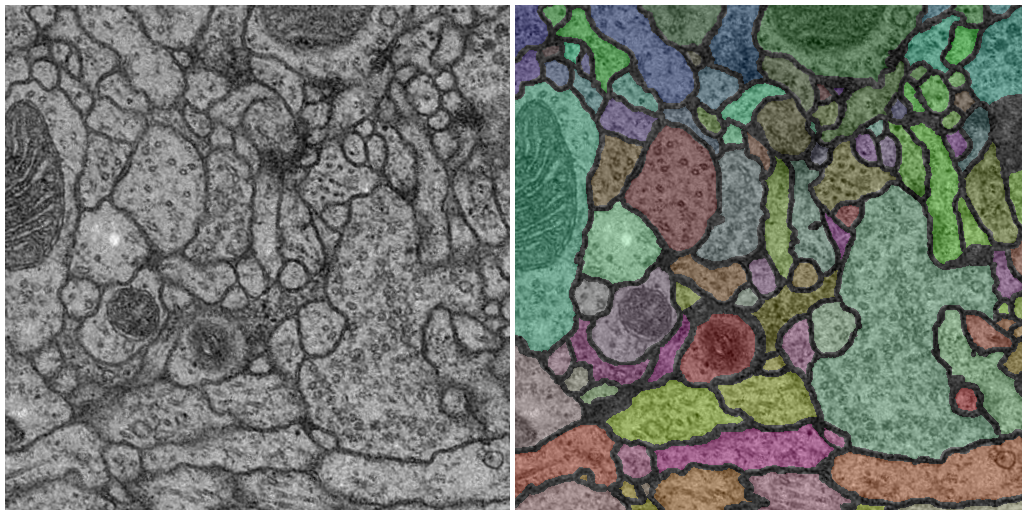
\includegraphics[width=\textwidth]{images/unet_original_dataset.png}
            \caption{Приклад сегментації на наборі даних ``ISBI Challenge: Segmentation of neuronal structures in EM stacks''. Набір із 30 розділів із серійного набору даних трансмісійної електронної мікроскопії (ssTEM) черевного нервового канатика (VNC) личинки першої стадії личинки дрозофіли. Маємо багато регіонів $\{\mathcal{P}_i\}$.}
        \end{figure}
    \end{frame}

    \begin{frame}{Ще приклади}
        \begin{figure}
            \centering
            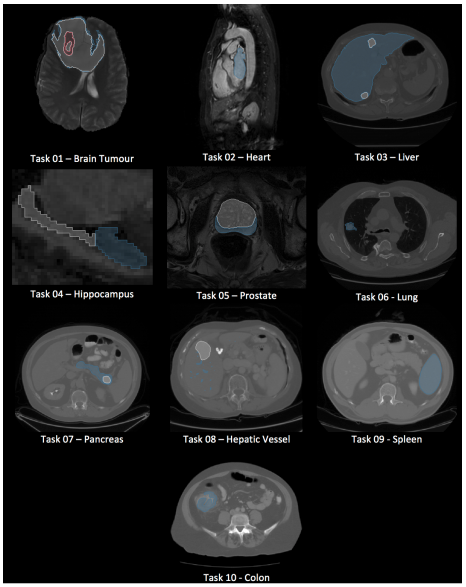
\includegraphics[width=0.75\textwidth]{images/decathlon.png}
        \end{figure}
    \end{frame}

    \subsection{Нейронні мережі: нагадування}
    \begin{frame}{Нейронні мережі}
        \begin{block}{Коротко}
            Нейронна мережа --- це параметризація функції
            $f(\boldsymbol{x}|\boldsymbol{\theta})$, що складається з 
            досить великої кількості параметрів $\boldsymbol{\theta} \in \mathbb{R}^n$.
        \end{block}

        \begin{example}
            Стандартні Fully Connected (FC) шари виглядають як:
            \begin{equation*}
                f(\boldsymbol{x}|\boldsymbol{\theta}) = \sigma \circ \boldsymbol{W}_{\ell} \circ \sigma \circ \boldsymbol{W}_{\ell-1} \circ \dots \circ \sigma \circ \boldsymbol{W}_1 \circ \boldsymbol{x},
            \end{equation*}
        \end{example}

        \begin{figure}
            \centering
            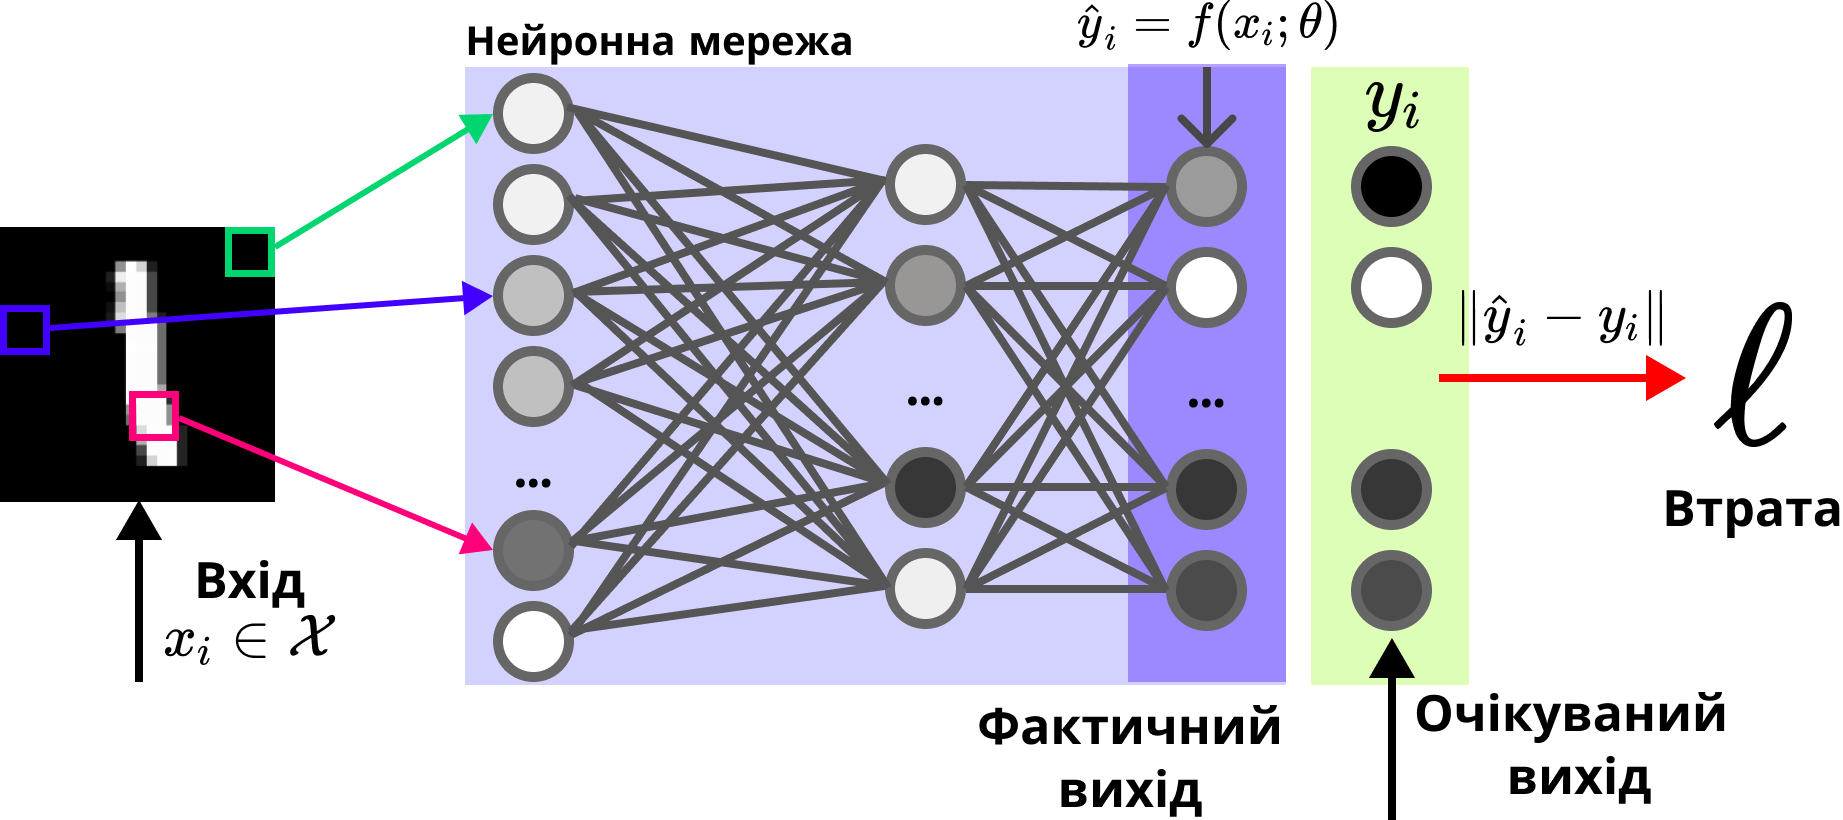
\includegraphics[width=0.6\textwidth]{images/full_forward_prop.png}
            \caption{Пряме поширення: обрахунок значення втрати}
        \end{figure}
    \end{frame}

    \begin{frame}{Конволюційна операція}
        \begin{figure}
            \centering
            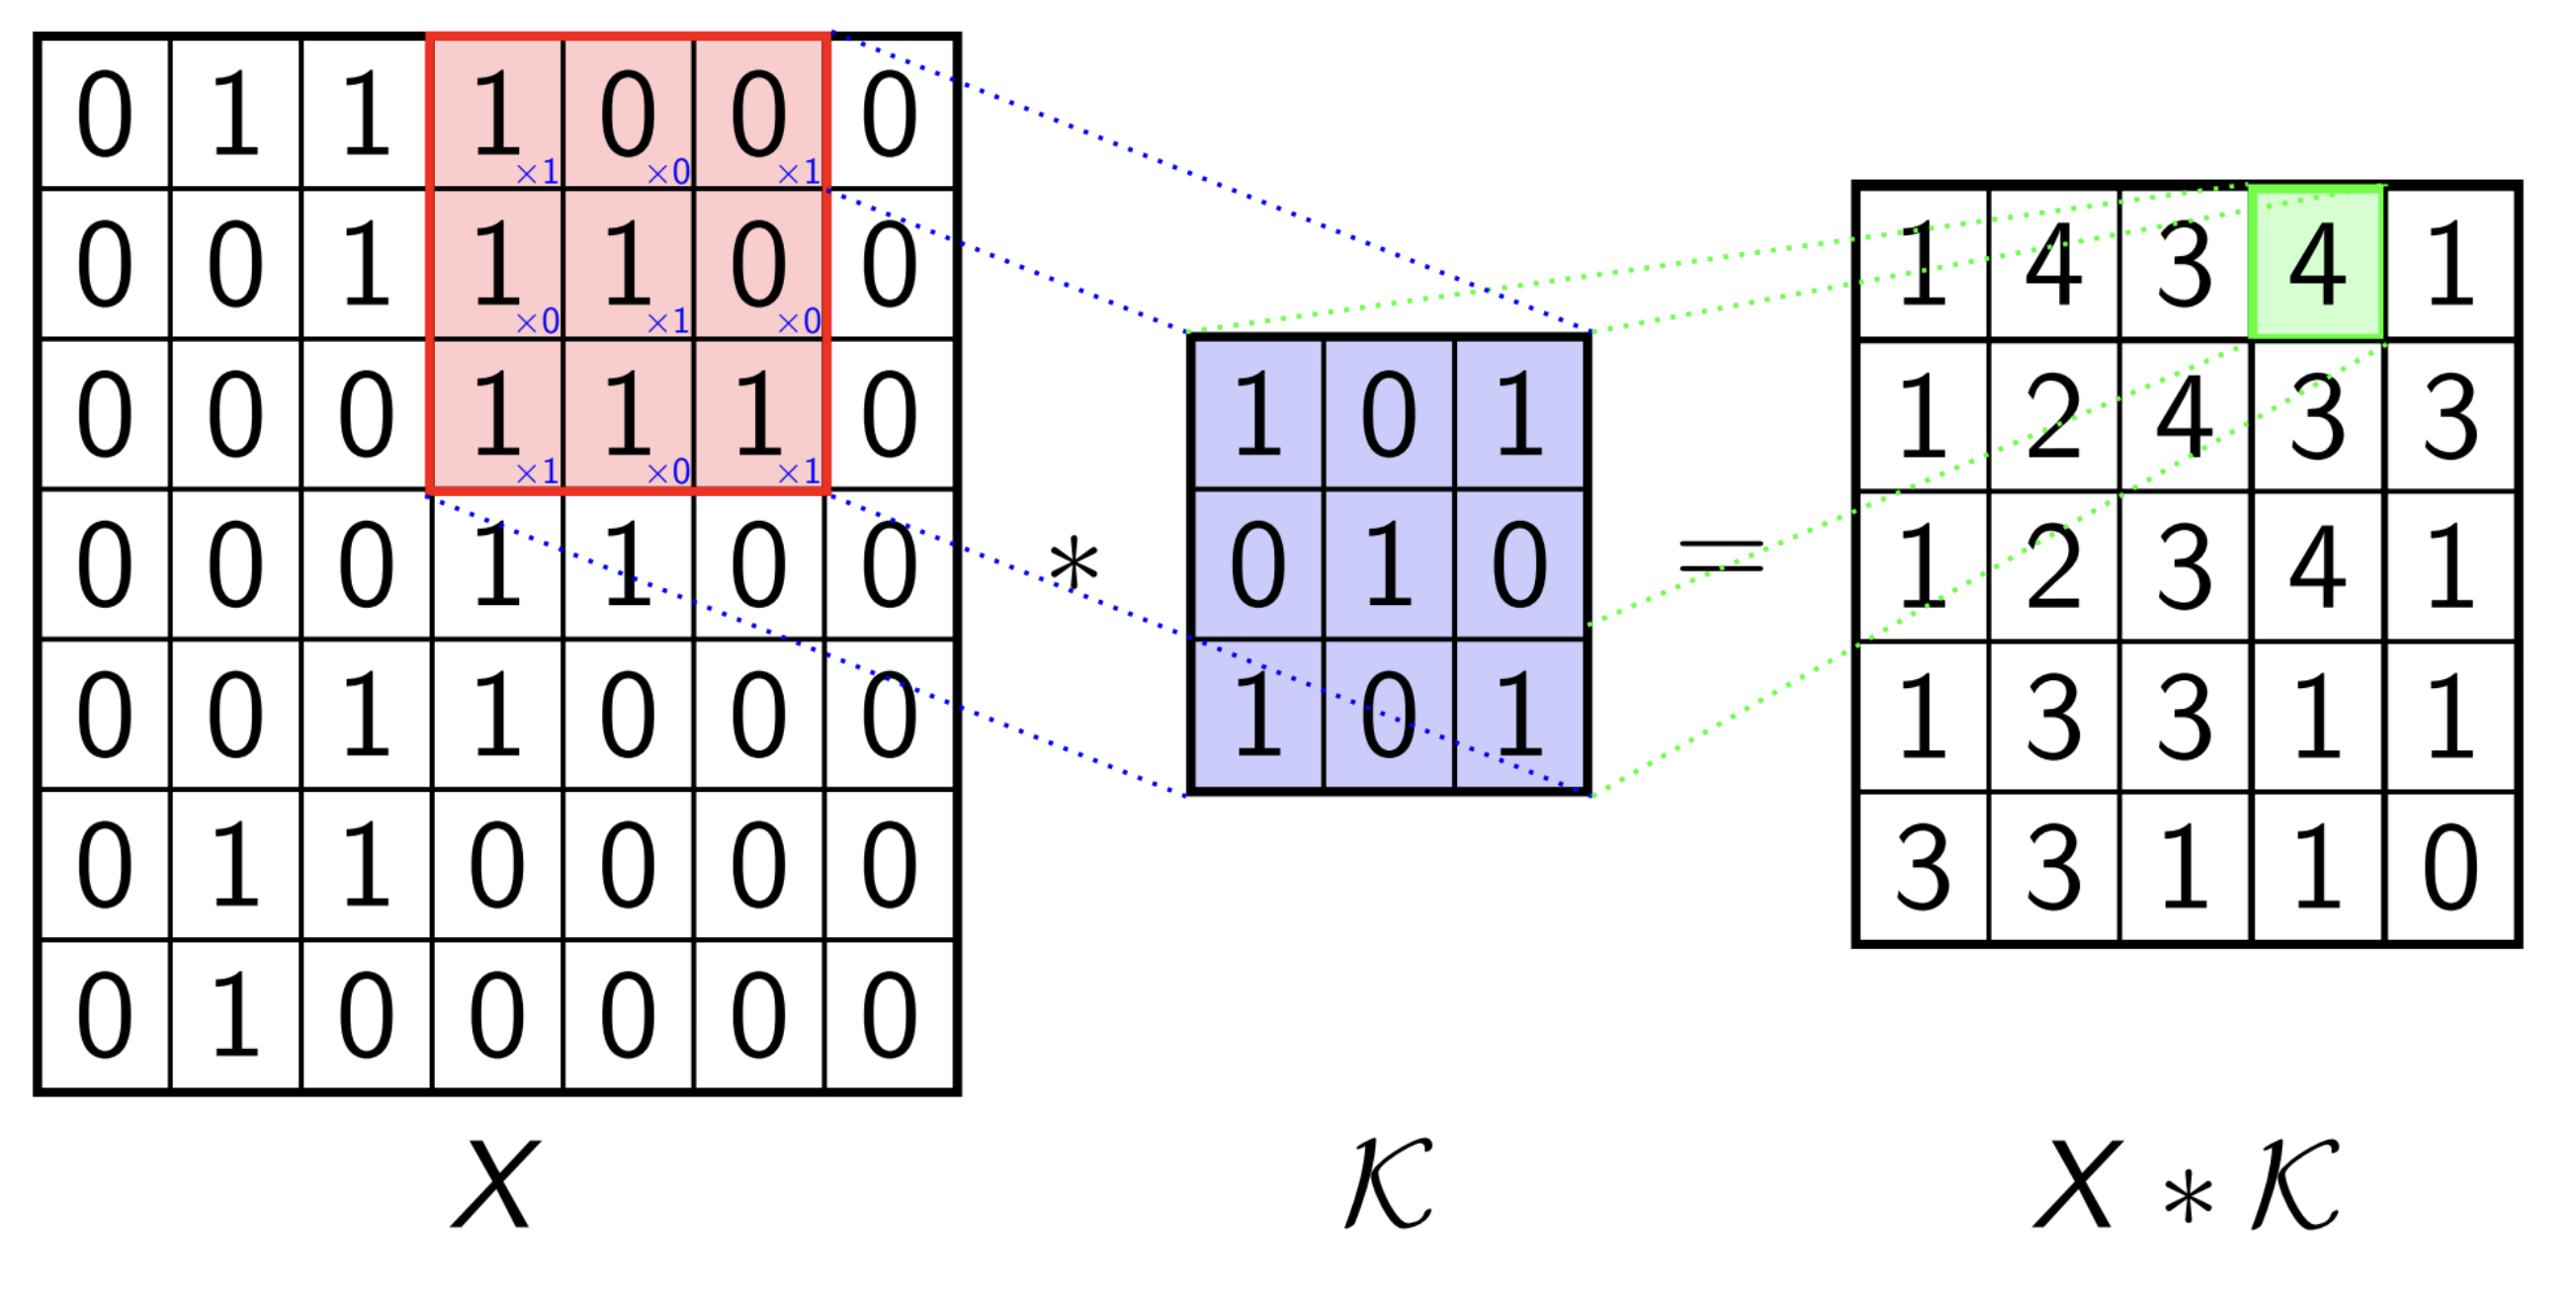
\includegraphics[width=\textwidth]{images/convolution.png}
            \caption{Механізм знаходження конволюції $X*\mathcal{K}$ для $\mathcal{K} \in \mathbb{R}^{3 \times 3}$ та $X \in \mathbb{R}^{7 \times 7}$.}
        \end{figure}
    \end{frame}

    \begin{frame}{Фільтри Собеля}
        \begin{figure}
            \centering
            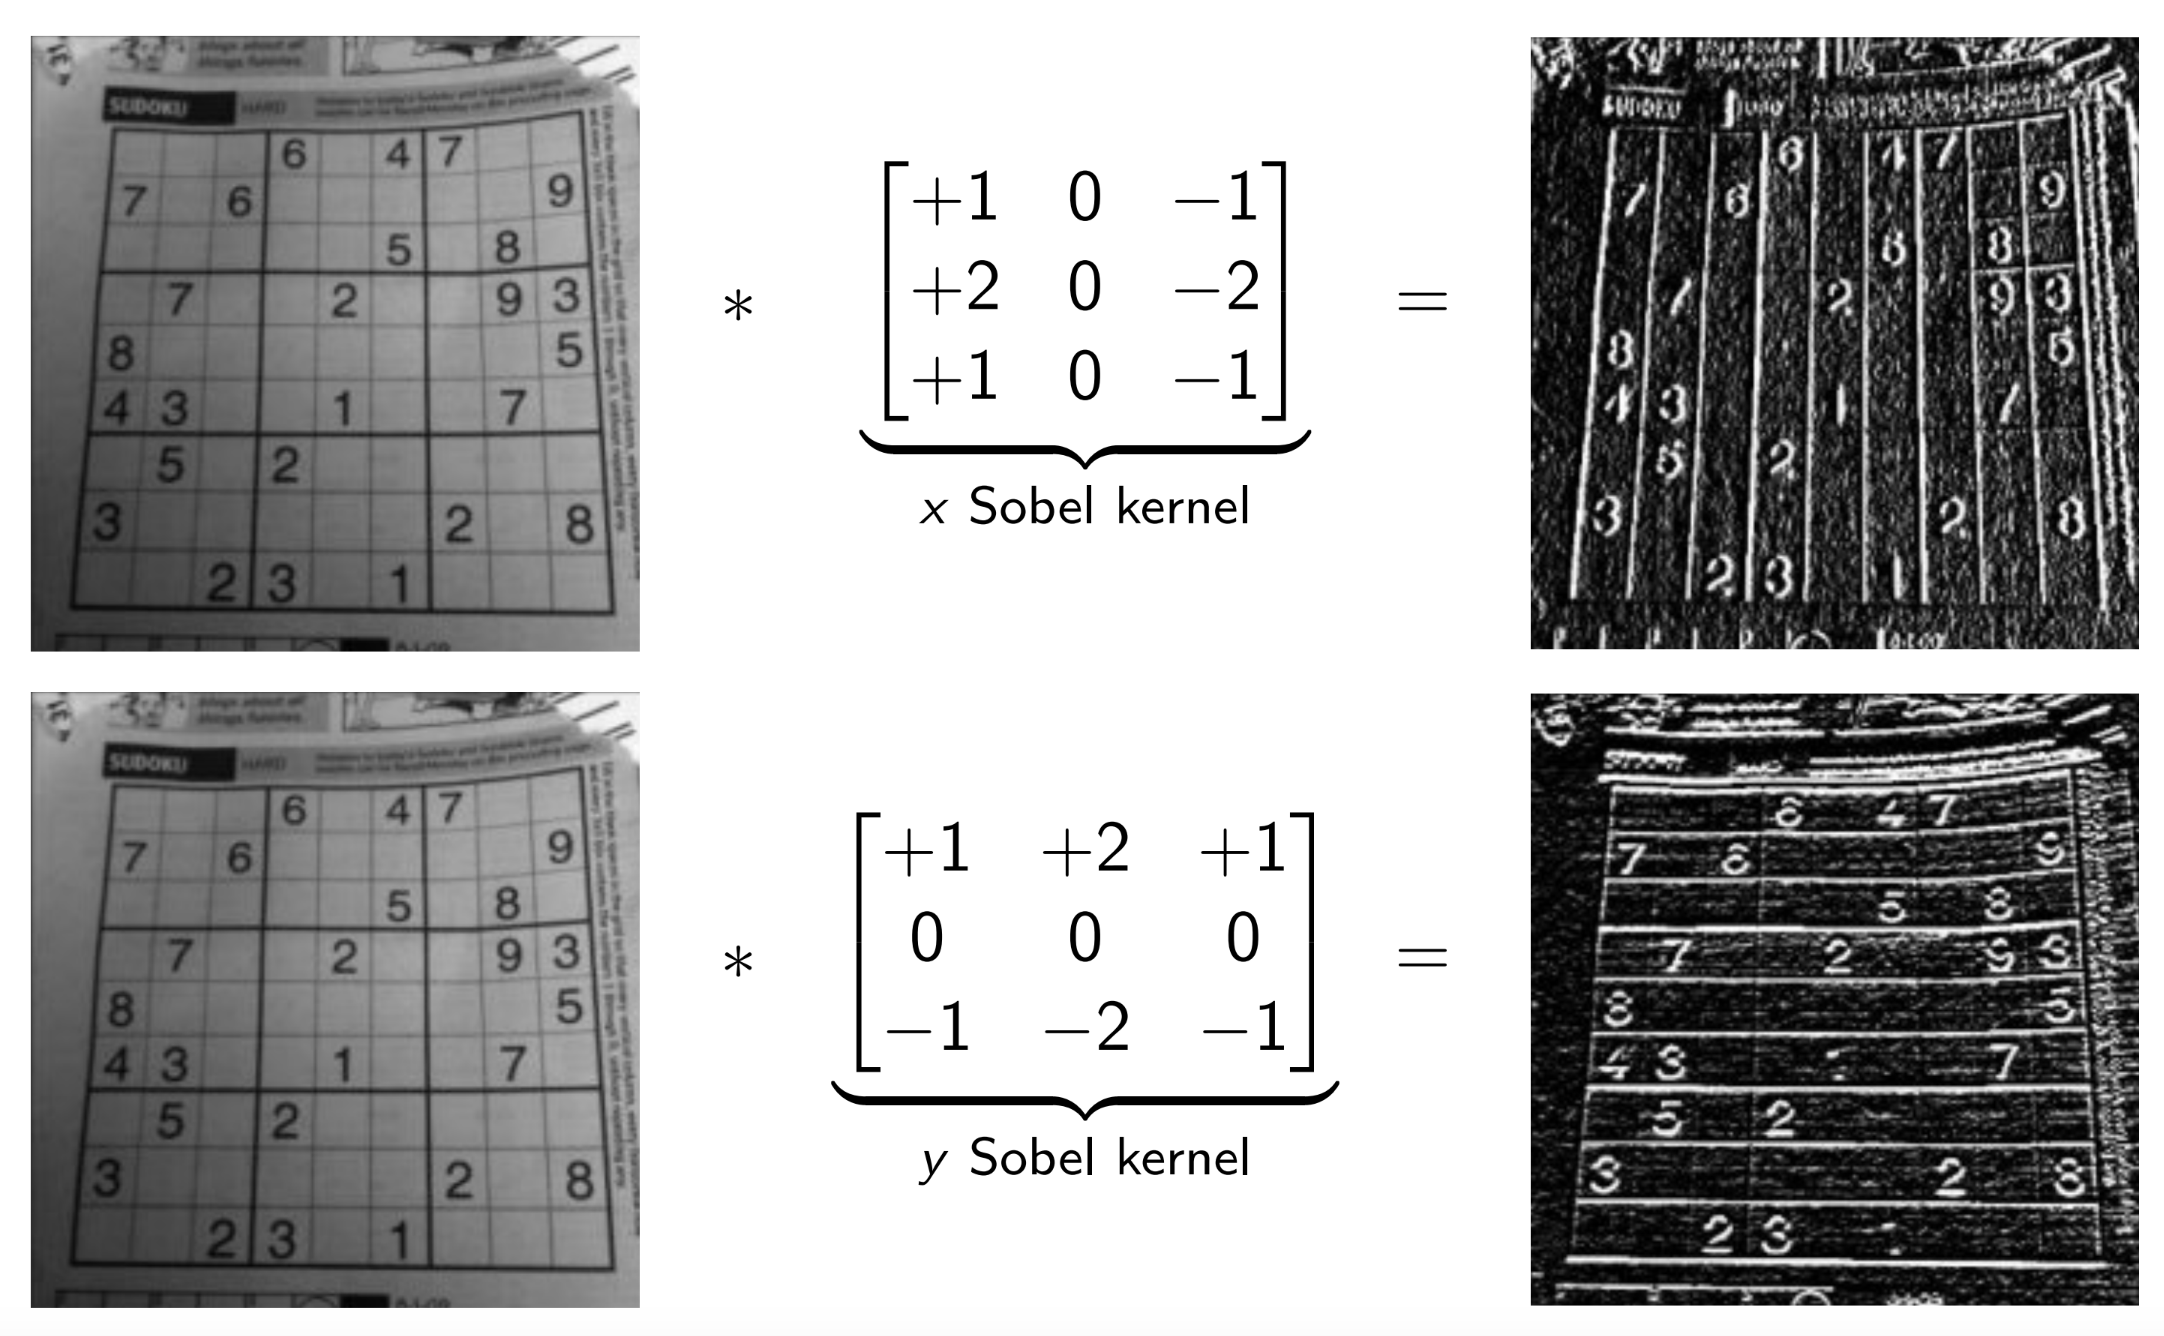
\includegraphics[width=\textwidth]{images/sobel.png}
            \caption{Демонстрація фільтрів Собеля.}
        \end{figure}
    \end{frame}

    \section{U-Net}

    \begin{frame}{Архітектура}
        \begin{block}{Ключова ідея}
            U-Net --- це так звана fully convolutional network модель, себто вона повністю 
            працює з зображеннями, не переходячи у виході на Fully Connected шари.
        \end{block}
        \begin{figure}
            \centering
            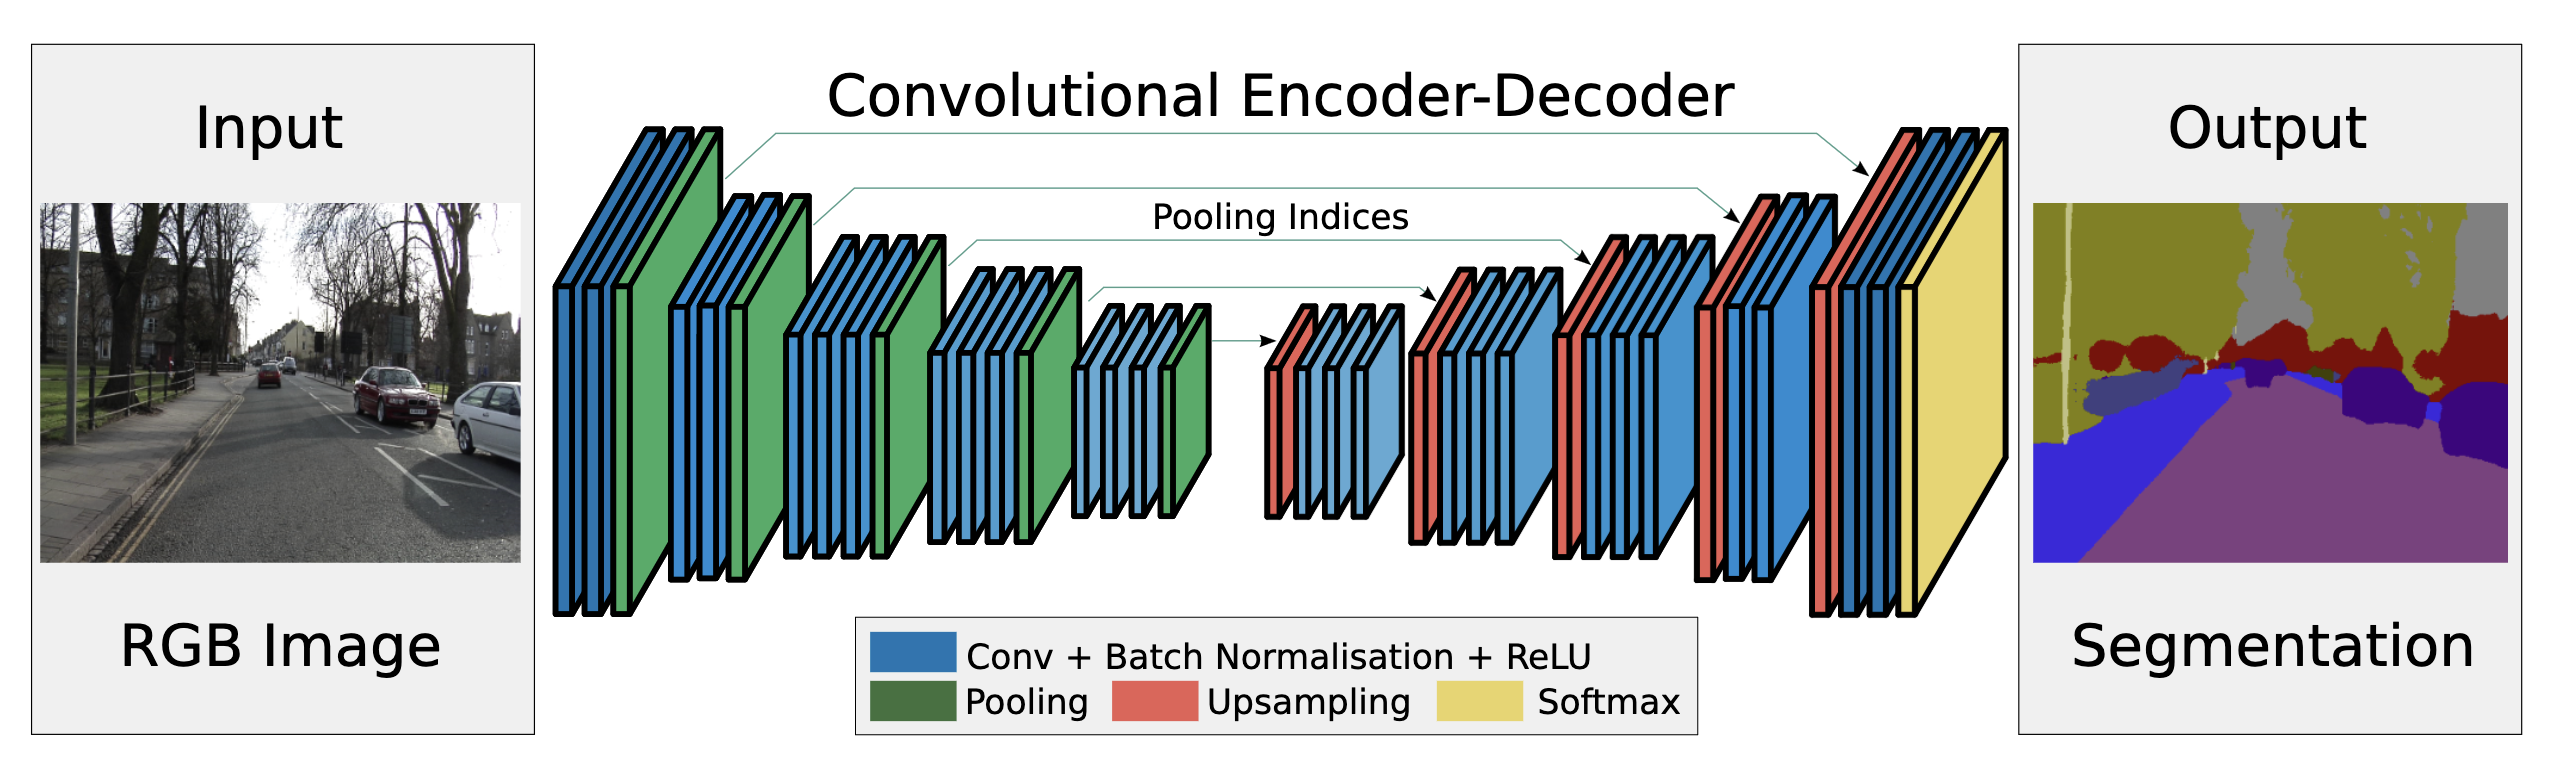
\includegraphics[width=\textwidth]{images/unet.png}
            \caption{Архітектура U-Net.}
        \end{figure}
    \end{frame}

    \begin{frame}{Тренування}
        Нехай $\Omega \subset \mathbb{Z}^2$ --- область на зображенні.
        \begin{definition}
            \textbf{Softmax} функцією називають вираз вигляду:
            \begin{equation*}
                p_k(\boldsymbol{x}) = \frac{\exp(a_k(\boldsymbol{x}))}{\sum_{k'=1}^K \exp(a_{k'}(\boldsymbol{x}))}.
            \end{equation*}
        \end{definition}

        \begin{definition}
            Функцією енергії називаємо вираз:
            \begin{equation*}
                E(\Omega | f) = \sum_{\boldsymbol{x} \in \Omega} w(\boldsymbol{x})\log p_{\ell(\boldsymbol{x})}(\boldsymbol{x}), \quad a_k(\boldsymbol{x}) = f(\boldsymbol{x})_k
            \end{equation*}

            де $w: \Omega \to \mathbb{R}$ --- вага пікселя, $\ell: \Omega \to [K]$ --- мітка пікселя.
        \end{definition}
    \end{frame}

    \begin{frame}{Тренування}
        \begin{definition}
            Мапою ваги називаємо вираз:
            \begin{equation*}
                w(\boldsymbol{x}) = w_c(\boldsymbol{x}) + w_0 \cdot \exp\left(-\frac{(d_1(\boldsymbol{x})+d_2(\boldsymbol{x}))^2}{2\sigma^2}\right),
            \end{equation*}
            де $w_c: \Omega \to \mathbb{R}$ --- мапа ваги для балансування, $d_1: \Omega \to \mathbb{R}$ --- відстань до границі найближчої клітинки, $d_2: \Omega \to \mathbb{R}$ --- відстань до границі другої за порядком клітинки іншого класу.
        \end{definition}

        \begin{figure}
            \centering
            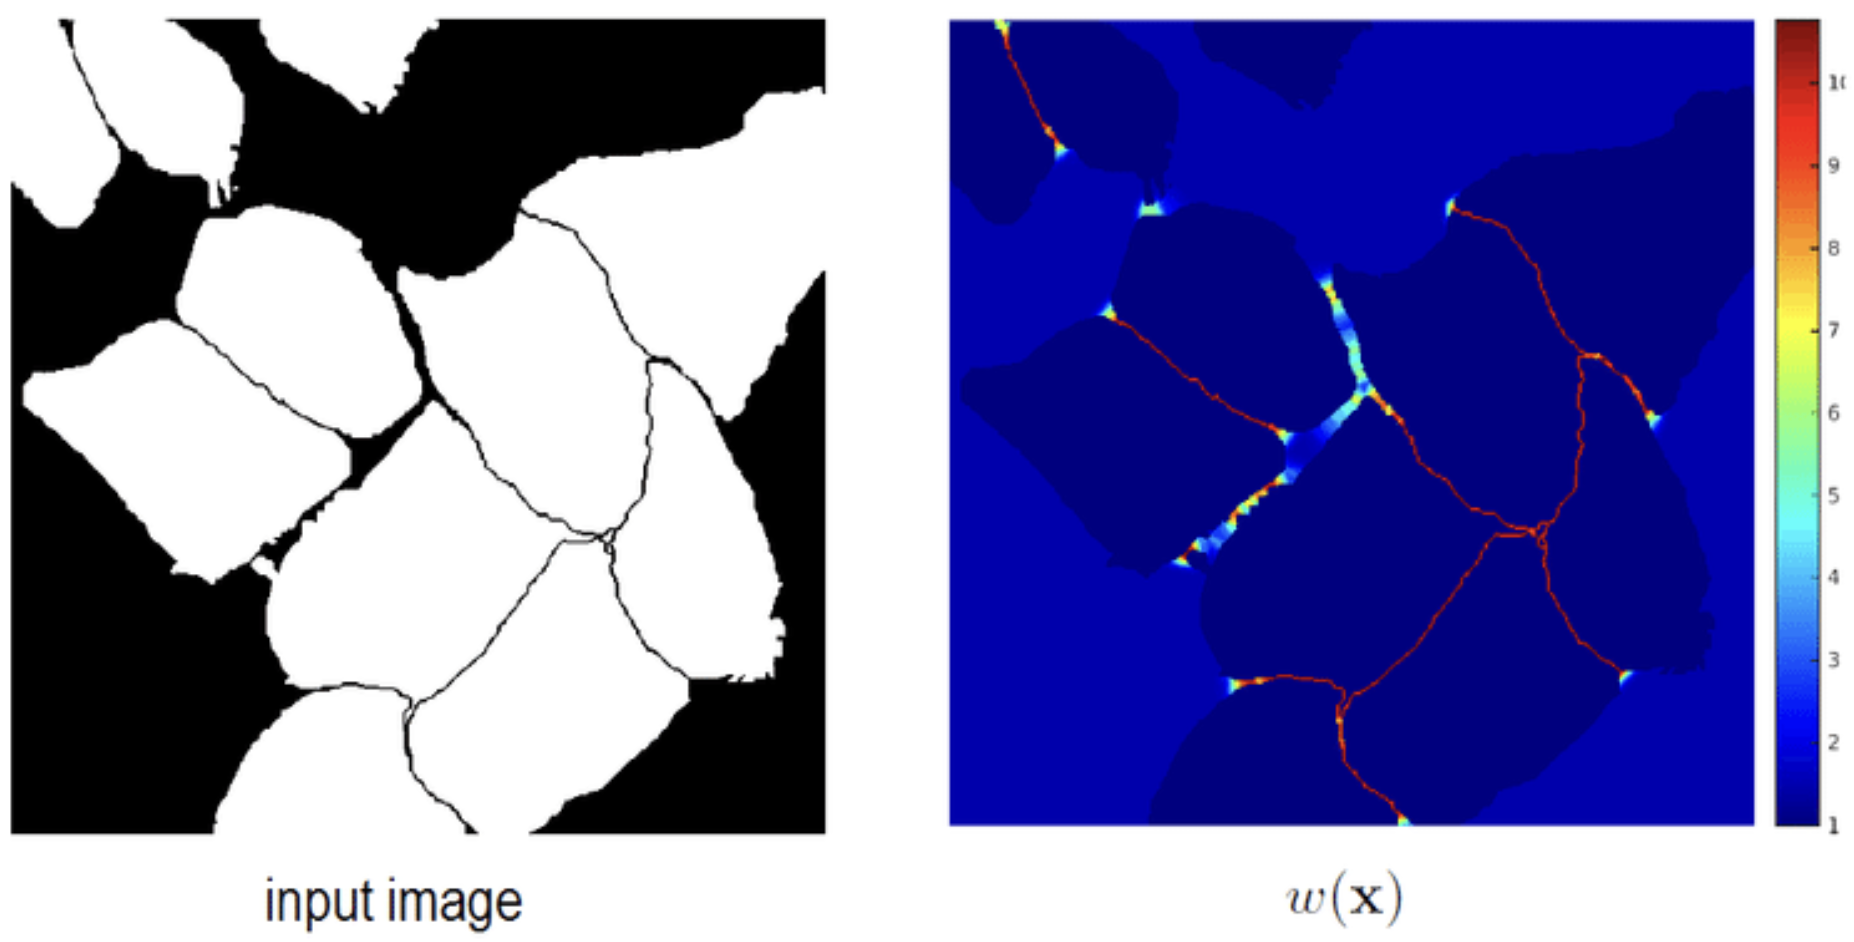
\includegraphics[width=0.6\textwidth]{images/unet_weightmap.png}
        \end{figure}
    \end{frame}

    \begin{frame}{Тренування}
        Наша нейронна мережа $f(X|\boldsymbol{\theta}): \mathbb{R}^{W \times H \times 3} \times \Theta \to [0,1]^{W \times H \times K}$. Таким чином,
        \begin{equation*}
            \hat{\boldsymbol{\theta}} = \arg\min_{\boldsymbol{\theta}} \frac{1}{N}\sum_{i=1}^N E(\Omega_i|f).
        \end{equation*}

        \begin{figure}
            \centering
            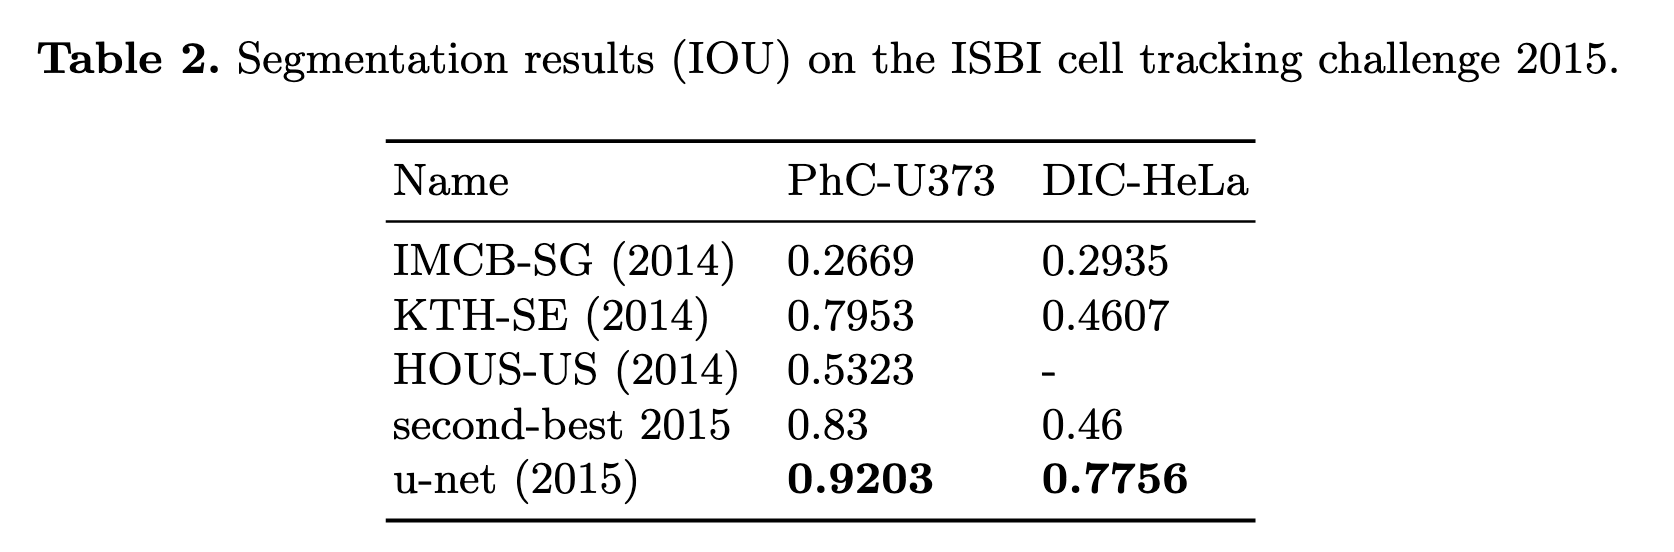
\includegraphics[width=\textwidth]{images/unet_results.png}
            \caption{Результат тренування U-Net.}
        \end{figure}
    \end{frame}
    
    \begin{frame}[plain, standout]
        \centering
        \LARGE
        \textbf{Дякую за Вашу Увагу!} \\
        
        \vspace{0.2cm} \Huge \ding{170} \large \\
    \end{frame}

\end{document}
